% unit: u05
% sources: sources/081-factorization-into-a-lu.txt, sources/132-factorization-into-a-lu.txt, sources/133-mit18-06scf11-ses1-4sum-pdf-download-file.txt, sources/134-lu-decomposition.txt, sources/135-mit18-06scf11-ses1-4prob-pdf-download-file.txt, sources/136-mit18-06scf11-ses1-4sol-pdf-download-file.txt
\section{Factorization into \texorpdfstring{\(A=LU\)}{A = LU}}\label{sec:u05}

Section~\ref{sec:u03} wrote elimination as $EA=U$, with $E$ a product of elimination
matrices. This section turns that statement around into $A=LU$: a lower triangular $L$ times
an upper triangular $U$. The surprise is that $L$ needs no computation at all; it simply
stores the multipliers. On the way we need the rules for inverting and transposing a product,
and afterwards we count how much work elimination costs (about $\tfrac13n^3$ operations)
and see what row exchanges do to the factorization.

\subsection{Inverses and transposes of products}

\begin{theorem}[Inverse of a product]\label{thm:u05-inv-product}
If $A$ and $B$ are invertible $n\times n$ matrices, then $AB$ is invertible and
\[
  (AB)^{-1}=B^{-1}A^{-1}.
\]
\end{theorem}

\begin{proof}
Using the associative law to regroup,
$(AB)(B^{-1}A^{-1})=A(BB^{-1})A^{-1}=AIA^{-1}=AA^{-1}=I$, and similarly
$(B^{-1}A^{-1})(AB)=B^{-1}(A^{-1}A)B=B^{-1}B=I$.
\end{proof}

The order reverses for the same reason as in everyday life: you put on socks, then shoes;
to undo it you take off the shoes first. The same holds for any number of factors:
$(ABC)^{-1}=C^{-1}B^{-1}A^{-1}$.

\begin{definition}[Transpose]\label{def:u05-transpose}
The \emph{transpose} of an $m\times n$ matrix $A$ is the $n\times m$ matrix $A\T$ whose rows
are the columns of $A$: $(A\T)_{ij}=a_{ji}$. For example
$\begin{bmatrix} 2 & 1\\ 8 & 7\end{bmatrix}\T=\begin{bmatrix} 2 & 8\\ 1 & 7\end{bmatrix}$.
\end{definition}

\begin{theorem}[Transpose of a product]\label{thm:u05-transpose-product}
If $AB$ is defined, then $(AB)\T=B\T A\T$. If $A$ is invertible, then so is $A\T$, and
$(A\T)^{-1}=(A^{-1})\T$.
\end{theorem}

\begin{proof}
Compare entries: $\bigl((AB)\T\bigr)_{ij}=(AB)_{ji}=\sum_k a_{jk}b_{ki}
=\sum_k (B\T)_{ik}(A\T)_{kj}=(B\T A\T)_{ij}$. For the second statement, transpose
$AA^{-1}=I$ using the first: $(A^{-1})\T A\T=I\T=I$. A one-sided inverse of a square matrix
is a true inverse (Corollary~\ref{cor:u04-onesided}), so $(A^{-1})\T$ is the inverse of $A\T$.
\end{proof}

So for a single matrix, inverting and transposing can be done in either order.

\subsection{From \texorpdfstring{\(EA=U\)}{EA = U} to \texorpdfstring{\(A=LU\)}{A = LU}}

\begin{example}[$LU$ and $LDU$ for a $2\times2$ matrix]\label{ex:u05-LU2}
The first pivot of $A=\begin{bmatrix} 2 & 1\\ 8 & 7\end{bmatrix}$
is $2$ and the multiplier is $\ell_{21}=8/2=4$:
\[
  \underbrace{\begin{bmatrix} 1 & 0\\ -4 & 1\end{bmatrix}}_{E_{21}}
  \underbrace{\begin{bmatrix} 2 & 1\\ 8 & 7\end{bmatrix}}_{A}
  =\underbrace{\begin{bmatrix} 2 & 1\\ 0 & 3\end{bmatrix}}_{U}.
\]
Multiply both sides on the left by $E_{21}^{-1}$, which \emph{adds} back $4$ times row~1:
\[
  \underbrace{\begin{bmatrix} 2 & 1\\ 8 & 7\end{bmatrix}}_{A}
  =\underbrace{\begin{bmatrix} 1 & 0\\ 4 & 1\end{bmatrix}}_{L}
  \underbrace{\begin{bmatrix} 2 & 1\\ 0 & 3\end{bmatrix}}_{U}.
\]
$L$ is lower triangular with ones on its diagonal and the multiplier $4$ below; $U$ is upper
triangular with the pivots $2,3$ on its diagonal. (Had the $7$ been a $4$, the second pivot
would have been $0$.) Sometimes it is useful to divide the pivots out of $U$ into a diagonal
matrix $D$, leaving ones on the diagonal of the last factor as well:
\[
  \begin{bmatrix} 2 & 1\\ 8 & 7\end{bmatrix}
  =\begin{bmatrix} 1 & 0\\ 4 & 1\end{bmatrix}
  \begin{bmatrix} 2 & 0\\ 0 & 3\end{bmatrix}
  \begin{bmatrix} 1 & \tfrac12\\ 0 & 1\end{bmatrix}
  \qquad (A=LDU).
\]
\end{example}

For a $3\times3$ matrix with no row exchanges, elimination is
$E_{32}E_{31}E_{21}A=U$, and inverting the three factors in reverse order gives
\[
  A=E_{21}^{-1}E_{31}^{-1}E_{32}^{-1}\,U=LU .
\]
Why prefer $L=E_{21}^{-1}E_{31}^{-1}E_{32}^{-1}$ to $E=E_{32}E_{31}E_{21}$?

\begin{example}[$E$ mixes the multipliers, $L$ keeps them]\label{ex:u05-EvsL}
Take $\ell_{21}=2$, $\ell_{31}=0$, $\ell_{32}=5$. Then
\[
  E=\underbrace{\begin{bmatrix} 1&0&0\\ 0&1&0\\ 0&-5&1\end{bmatrix}}_{E_{32}}
  \underbrace{\begin{bmatrix} 1&0&0\\ -2&1&0\\ 0&0&1\end{bmatrix}}_{E_{21}}
  =\begin{bmatrix} 1&0&0\\ -2&1&0\\ 10&-5&1\end{bmatrix},
  \qquad
  L=\underbrace{\begin{bmatrix} 1&0&0\\ 2&1&0\\ 0&0&1\end{bmatrix}}_{E_{21}^{-1}}
  \underbrace{\begin{bmatrix} 1&0&0\\ 0&1&0\\ 0&5&1\end{bmatrix}}_{E_{32}^{-1}}
  =\begin{bmatrix} 1&0&0\\ 2&1&0\\ 0&5&1\end{bmatrix}.
\]
The $10$ in $E$ appears because $2$ of row~1 went into row~2 and then $5$ of that row~2 went
into row~3, so row~1 reached row~3 with weight $10$. In $L$ the multipliers do not interfere:
they sit in their places untouched.
\end{example}

This is true in general.

\begin{theorem}[The multipliers go into $L$]\label{thm:u05-LU}
Suppose elimination on the $n\times n$ matrix $A$ succeeds without row exchanges, with
multipliers $\ell_{ij}$ ($i>j$) and upper triangular result $U$. Then $A=LU$, where $L$ is the
lower triangular matrix with ones on the diagonal and entry $\ell_{ij}$ in position $(i,j)$
below it.
\end{theorem}

\begin{proof}
Let $\vb{u}_j\T$ denote row $j$ of $U$. When elimination subtracts $\ell_{ij}$ times the pivot
row $j$ from row $i$, the pivot row is already finished (all its own eliminations used rows
above it and happened earlier), so what is subtracted is $\ell_{ij}\vb{u}_j\T$. Row $i$
undergoes these subtractions for $j=1,\dots,i-1$ and what remains is $\vb{u}_i\T$:
\[
  \vb{u}_i\T=(\text{row $i$ of }A)-\sum_{j<i}\ell_{ij}\vb{u}_j\T,
  \qquad\text{so}\qquad
  \text{row $i$ of }A=\sum_{j<i}\ell_{ij}\vb{u}_j\T+1\cdot\vb{u}_i\T .
\]
The right side is the combination of the rows of $U$ with weights from row $i$ of $L$, which
by the row view (Proposition~\ref{prop:u04-views}(b)) is row $i$ of $LU$.
\end{proof}

\begin{example}[$LU$ for the elimination example]\label{ex:u05-LU3}
For $A=\begin{bmatrix} 1&2&1\\ 3&8&1\\ 0&4&1\end{bmatrix}$ of Section~\ref{sec:u03} the
multipliers were $\ell_{21}=3$, $\ell_{31}=0$, $\ell_{32}=2$ and the pivots $1,2,5$. So
\[
  A=LU=\begin{bmatrix} 1&0&0\\ 3&1&0\\ 0&2&1\end{bmatrix}
  \begin{bmatrix} 1&2&1\\ 0&2&-2\\ 0&0&5\end{bmatrix}
  =\begin{bmatrix} 1&0&0\\ 3&1&0\\ 0&2&1\end{bmatrix}
  \begin{bmatrix} 1&&\\ &2&\\ &&5\end{bmatrix}
  \begin{bmatrix} 1&2&1\\ 0&1&-1\\ 0&0&1\end{bmatrix}.
\]
Check row~3 as in the proof: $0\,(1,2,1)+2\,(0,2,-2)+1\,(0,0,5)=(0,4,1)$, which is row~3 of
$A$. To solve $A\vb{x}=\vb{b}$ with $\vb{b}=(2,12,2)$, solve two triangular systems:
\begin{align*}
  L\vb{c}=\vb{b}&:\quad c_1=2,\quad c_2=12-3c_1=6,\quad c_3=2-0\cdot c_1-2c_2=-10;\\
  U\vb{x}=\vb{c}&:\quad 5z=-10,\quad 2y-2z=6,\quad x+2y+z=2\quad\Longrightarrow\quad (x,y,z)=(2,1,-2).
\end{align*}
The vector $\vb{c}$ is exactly the right-hand side that forward elimination produced in
Section~\ref{sec:u03}: solving $L\vb{c}=\vb{b}$ \emph{is} elimination applied to $\vb{b}$.
\end{example}

In a computer, $A$ can be overwritten as elimination proceeds: once row $i$ is finished, the
new row of $U$ and the multipliers $\ell_{ij}$ (which fill exactly the positions that became
zero) are all that must be kept. Nothing else about $A$ is needed again.

\begin{trap}
$L$ is not $E$ with its signs flipped. The matrix $E=L^{-1}$ can have extra entries, like
the $10$ above; only $L$ holds the plain multipliers. Also, ``$A=LU$ exists'' is about the
\emph{order of the rows}, not about invertibility: $\begin{bmatrix} 0&2\\ 3&4\end{bmatrix}$ is
invertible but has no $LU$ factorization (its first pivot position holds $0$), while a
singular matrix whose last pivot is $0$ still has one (Exercise~\ref{ex:u05-ab}).
\end{trap}

\subsection{How expensive is elimination?}

How long does a computer need to solve $n$ equations? Count the operations on a full
$n\times n$ matrix, taking one ``operation'' to be a multiplication or division, each paired
with at most one subtraction. The first stage clears column~1: for each of the $n-1$ rows
below the pivot it computes a multiplier and updates the other $n-1$ entries of the row, about
$n^2$ operations in all. The second stage does the same on the remaining
$(n-1)\times(n-1)$ block, about $(n-1)^2$ operations, and so on down to the last $1\times1$
block. The total is about
\[
  n^2+(n-1)^2+\cdots+2^2+1^2\;\approx\;\int_0^n x^2\,dx=\frac{n^3}{3}.
\]
Figure~\ref{fig:u05-cost} compares the sum with the integral. The exact count is just as
easy.

\begin{proposition}[Operation count]\label{prop:u05-count}
Without row exchanges, reducing an $n\times n$ matrix $A$ to $U$ takes exactly
$\tfrac13(n^3-n)$ operations (multiplications and divisions). Applying the same steps to one
right-hand side and back substituting takes $n^2$ operations.
\end{proposition}

\begin{proof}
At the stage with a $k\times k$ active block ($k=n,n-1,\dots,2$), each of the $k-1$ rows below
the pivot costs one division (its multiplier) and $k-1$ multiply-subtracts, so the stage
costs $(k-1)k$. Summing,
\[
  \sum_{k=1}^{n}(k^2-k)=\frac{n(n+1)(2n+1)}{6}-\frac{n(n+1)}{2}
  =\frac{n(n+1)(2n-2)}{6}=\frac{(n-1)n(n+1)}{3}=\frac{n^3-n}{3},
\]
using the standard formulas for $\sum k^2$ and $\sum k$. For the right-hand side, the stage
with a $k\times k$ block updates $k-1$ entries of $\vb{b}$, a total of
$\sum_{k}(k-1)=\tfrac12n(n-1)$. Back substitution for $x_i$ uses $n-i$ multiply-subtracts and
one division, a total of $\tfrac12n(n-1)+n$. Together that is $n(n-1)+n=n^2$.
\end{proof}

\begin{figure}[ht]
\centering
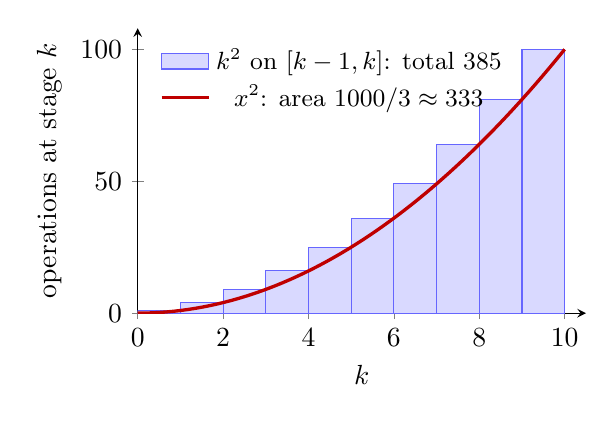
\begin{tikzpicture}
\begin{axis}[width=0.6\textwidth, height=5.2cm, xmin=0, xmax=10.5, ymin=0, ymax=108,
  xlabel={$k$}, ylabel={operations at stage $k$}, xtick={0,2,4,6,8,10},
  axis lines=left, legend pos=north west, legend style={font=\small,draw=none,fill=none}]
  \addplot[ybar interval, area legend, fill=blue!15, draw=blue!60] coordinates
    {(0,1) (1,4) (2,9) (3,16) (4,25) (5,36) (6,49) (7,64) (8,81) (9,100) (10,100)};
  \addlegendentry{$k^2$ on $[k-1,k]$: total $385$}
  \addplot[very thick, red!75!black, domain=0:10, samples=60] {x^2};
  \addlegendentry{$x^2$: area $1000/3\approx333$}
\end{axis}
\end{tikzpicture}
\caption{The work of elimination for $n=10$. Stage $k$ works on a $k\times k$ block and costs
about $k^2$ operations (bars). The bars and the parabola $x^2$ enclose nearly the same area,
so the total is about $\int_0^n x^2\,dx=n^3/3$. The exact count $\frac13(n^3-n)=330$ is even
closer, because the true cost of stage $k$ is $k^2-k$.}\label{fig:u05-cost}
\end{figure}

The cube matters. For $n=100$ elimination costs $\tfrac13(10^6-100)=333{,}300$ operations;
for $n=1000$ about $3.3\times10^8$. Doubling $n$ multiplies the work by $8$. Each additional
right-hand side costs only $n^2$, so a computer factors $A=LU$ once (the expensive part) and
then solves for many vectors $\vb{b}$ cheaply. Matrices with many zeros in good positions
(band matrices, for instance) cost far less, since zero entries need no elimination. By
contrast, the determinant formula with $n!$ terms (Section~\ref{sec:u21}) would be hopeless
for even $n=25$.

\subsection{Row exchanges and permutation matrices}

If a zero appears in a pivot position, elimination needs a row exchange, which is
multiplication by a permutation matrix (Definition~\ref{def:u03-perm}). For $3\times3$
matrices there are exactly six permutation matrices, one for each ordering of the rows of $I$:
\[
  I=\begin{bmatrix} 1&0&0\\ 0&1&0\\ 0&0&1\end{bmatrix},
  P_{12}=\begin{bmatrix} 0&1&0\\ 1&0&0\\ 0&0&1\end{bmatrix},
  P_{13}=\begin{bmatrix} 0&0&1\\ 0&1&0\\ 1&0&0\end{bmatrix},
  P_{23}=\begin{bmatrix} 1&0&0\\ 0&0&1\\ 0&1&0\end{bmatrix},
  \begin{bmatrix} 0&1&0\\ 0&0&1\\ 1&0&0\end{bmatrix},
  \begin{bmatrix} 0&0&1\\ 1&0&0\\ 0&1&0\end{bmatrix}.
\]
The first four leave rows alone or exchange one pair; the last two move all three rows in a
cycle (the fifth sends row~2 up to row~1, row~3 up to row~2 and row~1 down to row~3). The
family is closed: a product of two of them reorders rows twice, which is again a reordering,
and the inverse of each one is also in the list. The exchanges $P_{12},P_{13},P_{23}$ are their
own inverses, and the two cycles are inverses of each other. In every case the inverse is the
transpose, $P^{-1}=P\T$, a fact proved in Section~\ref{sec:u06}. There are $n!$ permutation
matrices of size $n$: $6$ for $n=3$ and $24$ for $n=4$.

With exchanges allowed, $A=LU$ becomes $PA=LU$: put the rows in a good order first, then
eliminate. The smallest example is $A=\begin{bmatrix} 0&2\\ 3&4\end{bmatrix}$. Its first pivot
position holds $0$, so exchange the rows: $P_{12}A=\begin{bmatrix} 3&4\\ 0&2\end{bmatrix}$,
which is already upper triangular, so $L=I$ and $U=P_{12}A$. Section~\ref{sec:u06} completes the
story with a $3\times3$ example.

\subsection{Exercises}

\begin{exercise}\label{ex:u05-EA}
Which matrix $E$ puts $A=\begin{bmatrix} 1&3&0\\ 2&4&0\\ 2&0&1\end{bmatrix}$ into triangular form
$EA=U$? Multiply by $E^{-1}=L$ to factor $A=LU$.
\end{exercise}
\begin{solution}
The multipliers are $\ell_{21}=2$ (row~2 becomes $(0,-2,0)$), $\ell_{31}=2$ (row~3 becomes
$(0,-6,1)$) and $\ell_{32}=-6/-2=3$ (row~3 becomes $(0,0,1)$). So
$U=\begin{bmatrix} 1&3&0\\ 0&-2&0\\ 0&0&1\end{bmatrix}$ and
\[
  E=E_{32}E_{31}E_{21}
  =\begin{bmatrix} 1&0&0\\ 0&1&0\\ 0&-3&1\end{bmatrix}
   \begin{bmatrix} 1&0&0\\ 0&1&0\\ -2&0&1\end{bmatrix}
   \begin{bmatrix} 1&0&0\\ -2&1&0\\ 0&0&1\end{bmatrix}
  =\begin{bmatrix} 1&0&0\\ -2&1&0\\ 4&-3&1\end{bmatrix}.
\]
(The $4$ is $-2-3\cdot(-2)$: row~3 lost $2$ of row~1 directly and gained $6$ of it through row~2.)
The inverse just collects the multipliers:
$L=E^{-1}=\begin{bmatrix} 1&0&0\\ 2&1&0\\ 2&3&1\end{bmatrix}$, and one checks
$LU=\begin{bmatrix} 1&3&0\\ 2&6-2&0\\ 2&6-6&1\end{bmatrix}=A$.
\end{solution}

\begin{exercise}\label{ex:u05-abcd}
Compute $L$ and $U$ for the symmetric matrix
$A=\begin{bmatrix} a&a&a&a\\ a&b&b&b\\ a&b&c&c\\ a&b&c&d\end{bmatrix}$. Find four conditions on
$a,b,c,d$ for $A=LU$ with four pivots.
\end{exercise}
\begin{solution}
Subtract row~1 from rows~2, 3 and~4 (multipliers $1$): the rows become
$(0,b-a,b-a,b-a)$, $(0,b-a,c-a,c-a)$, $(0,b-a,c-a,d-a)$. Subtract the new row~2 from rows~3
and~4 (multipliers $1$): $(0,0,c-b,c-b)$ and $(0,0,c-b,d-b)$. Subtract row~3 from row~4
(multiplier $1$): $(0,0,0,d-c)$. Hence
\[
  L=\begin{bmatrix} 1&0&0&0\\ 1&1&0&0\\ 1&1&1&0\\ 1&1&1&1\end{bmatrix},\qquad
  U=\begin{bmatrix} a&a&a&a\\ 0&b-a&b-a&b-a\\ 0&0&c-b&c-b\\ 0&0&0&d-c\end{bmatrix}.
\]
Four nonzero pivots, with no row exchanges, require $a\neq0$, $b\neq a$, $c\neq b$ and
$d\neq c$.
\end{solution}

\begin{trap}
The posted solution to this problem lists the last condition as $d=c$. That is a slip: with
$d=c$ the fourth pivot $d-c$ is zero. The four conditions are all inequalities.
\end{trap}

\begin{exercise}\label{ex:u05-ab}
Find the $LU$ factorization of $A=\begin{bmatrix} 1&0&1\\ a&a&a\\ b&b&a\end{bmatrix}$ when it
exists. For which real numbers $a,b$ does it exist?
\end{exercise}
\begin{solution}
Step $(2,1)$: $\ell_{21}=a$, row~2 becomes $(0,a,0)$. Step $(3,1)$: $\ell_{31}=b$, row~3
becomes $(0,b,a-b)$. Step $(3,2)$ needs the pivot $a$ to be nonzero; then $\ell_{32}=b/a$ and
row~3 becomes $(0,0,a-b)$. So, for $a\neq0$,
\[
  A=\begin{bmatrix} 1&0&0\\ a&1&0\\ b&b/a&1\end{bmatrix}
    \begin{bmatrix} 1&0&1\\ 0&a&0\\ 0&0&a-b\end{bmatrix}.
\]
If $a=0$, row~2 of the partly reduced matrix is zero while row~3 is $(0,b,-b)$; for $b\neq0$
a row exchange is required, and for $b=0$ there is no pivot in column~2 at all. Either way
there is no $LU$ factorization with a nonzero second pivot, so the condition is $a\neq0$.
The third pivot $a-b$ may be zero: for $a=b\neq0$ the matrix is singular, yet $A=LU$
exists, because no row exchange was needed to reach $U$. Always check by multiplying: row~3
of $LU$ is $b(1,0,1)+\tfrac ba(0,a,0)+(0,0,a-b)=(b,b,a)$.
\end{solution}

\begin{exercise}\label{ex:u05-time}
A computer performs $10^9$ operations per second. Using Proposition~\ref{prop:u05-count},
estimate the time to factor a full $1000\times1000$ matrix, the time for each additional
right-hand side, and the time to factor a $10{,}000\times10{,}000$ matrix.
\end{exercise}
\begin{solution}
For $n=1000$: $\tfrac13(10^9-10^3)\approx3.3\times10^8$ operations, about $0.33$ seconds.
Each right-hand side then costs $n^2=10^6$ operations, one millisecond. For $n=10^4$ the
factorization costs about $\tfrac13\times10^{12}$ operations, roughly $333$ seconds or five
and a half minutes: ten times the size, a thousand times the work. (Real machines are faster,
and sparse matrices are much cheaper, but the $n^3$ growth is the same.)
\end{solution}
